%% V1.0
%% by Pritesh Gudge, priteshgudge@gmail.com
%% 

%% Be Udacious!

\documentclass[10pt,journal,compsoc]{IEEEtran}

\usepackage[pdftex]{graphicx}    
\usepackage{cite}
\hyphenation{op-tical net-works semi-conduc-tor}
\usepackage{hyperref}
\usepackage{enumerate}

\begin{document}

\title{Adaptive Monte Carlo Localization Project}

\author{Pritesh Gudge}

\markboth{Localization project, Robotics Nanodegree Program, Udacity}%
{}
\IEEEtitleabstractindextext{%

\begin{abstract}
The project includes the application of the AMCL Package in ROS for localization and using sensor fusion of an Odometer and a Hokuyo Laser Range Finder in a Gazebo Simulation Environment. Two Robots with different configurations are used simulated in Gazebo for the project.The simulated robot is supposed to navigate in a controlled obstacle simulation by continuously localizing its pose on the global map and building a cost map to calculate further trajectory in order to be able to reach the goal location without getting stuck and by using the shortest route possible. 
\end{abstract}

% Note that keywords are not normally used for peerreview papers.
\begin{IEEEkeywords}
Robot, IEEEtran, Udacity, Localization, Monte Carlo Localization.
\end{IEEEkeywords}}


\maketitle
\IEEEdisplaynontitleabstractindextext
\IEEEpeerreviewmaketitle
\section{Introduction}
\label{sec:introduction}

\IEEEPARstart{T}{he} real world mobile robots always have to perform certain actions based on the tasks they are supposed to perform. The next action of the robot is based on the position on the robot in the operating environment and the task to be performed. The project attempts to implement Adaptive Monte Carlo Localization\cite{amcl} for a simulated environment. The base environment provided by Udacity is used here. ROS AMCL package is used to for the localization. The decisions about the actuation robot are based on the sensor fusion data fed into the AMCL algorithm and the corresponding outputs.


\section{Background}
For a robot to operate in the real world, it needs to keep track of its position and orientation, also called pose. The robots needs to continuously calculate its pose to be able to perform its movement and tasks. This is called the localization problem.

Robot Localization problems are classified on the complexity of the localization task and the environment. Position Tracking, Global Localization and Kidnapped Robot Localization.
Due to the uncertainties in measurement and real world operation scenarios the robot's position and the related actuation required also has uncertainty. Filters and localization algorithms are used to solve some of the problems. Robots operating in the real world have to adapt the terrain, location and displacement from predefined paths. The robots should be able to recover and continue functioning effectively.

\subsection{Kalman Filters}
Kalman filters work by performing state prediction, followed by measurement update from multiple sensors(also called sensor fusion). The measurement update with the previous state provides an estimate of the next state of the robot. The Kalman filters take into account the uncertainty in measurement of the sensors and performs state prediction by using the previous state and measurement update.
 
The assumptions of Kalman filters are: motion and measurement models are linear, state space can be represented by a unimodal Gaussian distribution. These assumptions cannot be applied to all the real world robots where motion and measurement models are complex non-linear curves and states cannot be modelled as unimodal Gaussian distribution.


The Extended Kalman Filters can be used to when the motion or measurement functions are non-linear. The non-linear functions can be used to update the mean but not the variance. Over a short interval of time, non-linear functions can be approximated to locally linear functions by using the Taylor series equation. Thus, Taylor series\cite{taylor} can be used to provide approximate state and measurement updates for the variance. 


Briefly describe Kalman filters. Explain how they work and why they are used for localization. Additionally, discuss the drawbacks of linear Kalman filters and how Extended Kalman Filters (EKFs) help resolve some of these issues.

\subsection{Particle Filters}
In robotics, a particle is a virtual element that represents a robot's pose. The particles are sampled at each movement of the robot. Monte Carlo Localization Algorithm is called Particle Filter Algorithm. This works only for Global Localization problems.
The powerful Monte Carlo localization algorithm estimates the posterior distribution of a robot’s position and orientation based on sensory information. This process is known as a recursive Bayes filter


\subsection{Comparison / Contrast}
The differences between the EKF and MCL(Particle Filter) approaches are described below.

%example for Bullet point list
\subsubsection{EKF}
\begin{itemize}
\item EKF is memory and computationally efficient algorithm.
\item EKF can effectively model Unimodal Continuous State Spaces.
\item EKF can be used in Position Tracking Localization Problems
\item EKF cannot be used to solve Global Localization Problem
\item EKF is relatively difficult to implement due to the complex equations involved to code.
\item For larger problems the memory and resolution cannot be controlled. 
\end {itemize}

\subsubsection{MCL}
\begin{itemize}
\item MCL is memory and computationally heavy algorithm.
\item MCL can effectively model Multimodal Discrete State Spaces.
\item MCL can be used to solve Global Localization Problem
\item MCL is relatively easy to implement.
\item For larger problems the memory and resolution can be controlled. 
\item MCL is robust and can recover from errors and wrong estimations.
\end {itemize}

\section{Simulations}
The simulation is performed in the Gazebo Physics simulator environment. The simulation is done with the provided benchmark robot and a custom robot. The simulation is aimed at reaching a pre-defined target by performing simultaneous localization and motion until the robot reaches the final goal pose.

\subsection{Achievements}
% Robot Models
\subsection{Benchmark Model}
\subsubsection{Model design}
The project has a base model provided for benchmarking and parameter setting for evaluation. 

\begin{figure}[thpb]
      \centering
      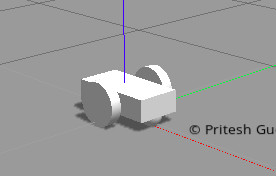
\includegraphics[width=\linewidth]{images/basic_setup1}
      \caption{Benchmark Model}
      \label{fig:benchmarkmodel}
\end{figure}

%example for building table
\begin{table}[h]
\caption{ Benchmark Model}
\label{benchmarkmodeltable}
\begin{center}
\begin{tabular}{|c|c|}
\hline
Property & Values\\
\hline
Length & 0.4m \\
\hline
Width & 0.2m \\
\hline
Heigth & 0.1m \\
\hline
Mass & 15 kg \\
\hline
Wheel Radius & 0.1m \\
\hline
Castor Radius & 0.05m \\
\hline
Camera & Front of Chassis (x=0.2m) \\
\hline
Hokuyo Depth Sensor & Top of Chassis (x=0.15m \& z=0.1m) \\
\hline
\end{tabular}
\end{center}
\end{table}


\subsubsection{Packages Used}
The following Packages were used:
\begin{enumerate}[i]
\item Camera: Topic- \begin{verbatim} "/udacity_bot/camera1/image_raw" 
\end{verbatim} 
\item Depth Sensor(Hokuyo): Topic-  \begin{verbatim}  "/udacity_bot/laser/scan" 
\end{verbatim}
\item Move Base Package Reads the config parameters and controls the cmd\_vel topic. It reads from the odom and depth sensor topics. 
\item AMCL Package Reads the Config Parameters. Reads the Odom and Depth Sensor Topics and writes out the robots estimated state.
\item Robot State Publisher Publishes the robots pose
\item Joint State Publisher Publishes the robots joint states
\end{enumerate}

\iffalse
The packages used in the project should be specified as well as the topics received and published; the services it used and provided should also be addressed. 
The amcl package 
\fi

\subsubsection{Parameters}
\iffalse
Localization parameters in the AMCL node should be described, as well as move\_base parameters in the configuration file. You should be able to clearly demonstrate your understanding of the impact of these parameters.
\fi
\begin{itemize}
\item AMCL \begin{itemize}
\item	min\_particles: 10
\item max\_particles: 50
\item transform\_tolerance: 0.3
\item controller\_frequency: 15
\item odom\_alpha(all): 0.01
\end{itemize}

\item local\_costmap
\begin{itemize}
 \item  global\_frame: odom
 \item  robot\_base\_frame: robot\_footprint
 \item  update\_frequency: 20.0
  \item publish\_frequency: 15.0
 \item  width: 5.0
 \item  height: 5.0
 \item  resolution: 0.1
 \item  static\_map: false
  \item rolling\_window: true
\end{itemize}

\item global\_costmap
\begin{itemize}
  \item robot\_base\_frame: robot\_footprint
  \item update\_frequency: 20.0
  \item publish\_frequency: 15.0
  \item width: 80.0
  \item height: 80.0
  \item resolution: 0.1
  \item static\_map: true
  \item rolling\_window: false
\end{itemize}


\item costmap\_common
\begin{itemize}
\item obstacle\_range: 2.5
\item raytrace\_range: 3.0

\item transform\_tolerance: 0.3

\item robot\_radius: 0.2
\item inflation\_radius: 0.1

\item observation\_sources: laser\_scan\_sensor

\item pdist\_scale: 2.0
\item gdist\_scale: 3.3
\item occdist\_scale: 1.5

\item meter\_scoring: true

\item sim\_time: 2.0


\item xy\_goal\_tolerance: 0.05
\item yaw\_goal\_tolerance: 0.05

\end{itemize}


\item TrajectoryPlannerROS
\begin{itemize}
\item   holonomic\_robot: false
 \item  acc\_lim\_x: 2.0
  \item acc\_lim\_y: 2.0

 \item  acc\_lim\_theta: 1.5

  \item min\_vel\_theta: -0.4
  \item max\_vel\_theta: 0.4

  \item max\_vel\_x: 0.4
  \item min\_vel\_x: -0.4
  
  \item escape\_vel: -0.3
  

  \item xy\_goal\_tolerance: 0.05
  \item yaw\_goal\_tolerance: 0.05
\end{itemize}

\end{itemize}

\subsection{Custom Model}
% ditto
\subsubsection{Model design}
The model is designed using a chassis with two wheels in the rear connected by a differential drive controller. On the front a smooth caster is placed for support and easy turn manoeuvring. Refer figure \ref{fig:custommodel}

\begin{figure}[thpb]
      \centering
      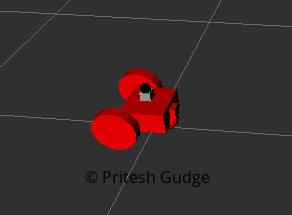
\includegraphics[width=\linewidth]{images/custom_obj}
      \caption{Custom Model}
      \label{fig:custommodel}
\end{figure}

\begin{table}[h]
\caption{ Custom Model}
\label{custommodeltable}
\begin{center}
\begin{tabular}{|c|c|}
\hline
Property & Values\\
\hline
Length & 0.2m \\
\hline
Width & 0.2m \\
\hline
Heigth & 0.1m \\
\hline
Mass & 10 kg \\
\hline
Wheel Radius & 0.1m \\
\hline
Castor Radius & 0.05m \\
\hline
Camera & Front of Chassis (x=0.1m) \\
\hline
Hokuyo Depth Sensor & Top of Chassis (z=0.1m) \\
\hline
\end{tabular}
\end{center}
\end{table}


\subsubsection{Packages Used}
The following Packages were used:
\begin{enumerate}[i]
\item Camera: Topic- \begin{verbatim} "/udacity_bot/camera1/image_raw" 
\end{verbatim} 
\item Depth Sensor(Hokuyo): Topic-  \begin{verbatim}  "/udacity_bot/laser/scan" 
\end{verbatim}
\item Move Base Package Reads the config parameters and controls the cmd\_vel topic. It reads from the odom and depth sensor topics. 
\item AMCL Package Reads the Config Parameters. Reads the Odom and Depth Sensor Topics and writes out the robots estimated state.
\item Robot State Publisher Publishes the robots pose
\item Joint State Publisher Publishes the robots joint states
\end{enumerate}

\subsubsection{Parameters}
\begin{itemize}
\item AMCL \begin{itemize}
\item	min\_particles: 10
\item max\_particles: 50
\item transform\_tolerance: 0.3
\item controller\_frequency: 15
\item odom\_alpha(all): 0.1
\end{itemize}

\item local\_costmap
\begin{itemize}%
 \item  global\_frame: odom
 \item  robot\_base\_frame: robot\_footprint
 \item  update\_frequency: 20.0
  \item publish\_frequency: 15.0
 \item  width: 5.0
 \item  height: 5.0
 \item  resolution: 0.1
 \item  static\_map: false
  \item rolling\_window: true
\end{itemize}

\item global\_costmap
\begin{itemize}
  \item robot\_base\_frame: robot\_footprint
  \item update\_frequency: 20.0
  \item publish\_frequency: 15.0
  \item width: 90.0
  \item height: 90.0
  \item resolution: 0.1
  \item static\_map: true
  \item rolling\_window: false
\end{itemize}


\item costmap\_common
\begin{itemize}
\item obstacle\_range: 2.5
\item raytrace\_range: 3.0

\item transform\_tolerance: 0.3

\item robot\_radius: 0.2
\item inflation\_radius: 0.1

\item observation\_sources: laser\_scan\_sensor

\item pdist\_scale: 2.5
\item gdist\_scale: 1.5
\item occdist\_scale: 1.6

\item meter\_scoring: true

\item sim\_time: 1.5

\item xy\_goal\_tolerance: 0.05
\item yaw\_goal\_tolerance: 0.05

\item oscillation\_reset\_dist: 0.01

\end{itemize}

\item TrajectoryPlannerROS
\begin{itemize}
\item   holonomic\_robot: false
 \item  acc\_lim\_x: 2.0
  \item acc\_lim\_y: 2.0

 \item  acc\_lim\_theta: 1.5

  \item min\_vel\_theta: -0.4
  \item max\_vel\_theta: 0.4

  \item max\_vel\_x: 0.4
  \item min\_vel\_x: -0.4
  
  \item escape\_vel: -0.3
  

  \item xy\_goal\_tolerance: 0.05
  \item yaw\_goal\_tolerance: 0.05
\end{itemize}
\end{itemize}



\section{Results}

\subsection{Localization Results}
The below sections describe the results of the AMCL run on the benchmark and the custom models. 

\subsubsection{Benchmark}
The benchmark model reaches the destination with a position tolerance set at 0.05 metres and orientation tolerance set at 0.05 radians. The path taken is show in figure and figure \ref{fig:benchresult3}, figure \ref{fig:benchresult4} and figure \ref{fig:benchresult5}. The model smoothly reaches the goal.  The output image is described in the figure \ref{fig:benchresult1}.
%example for inserting image
\begin{figure}[thpb]
      \centering
      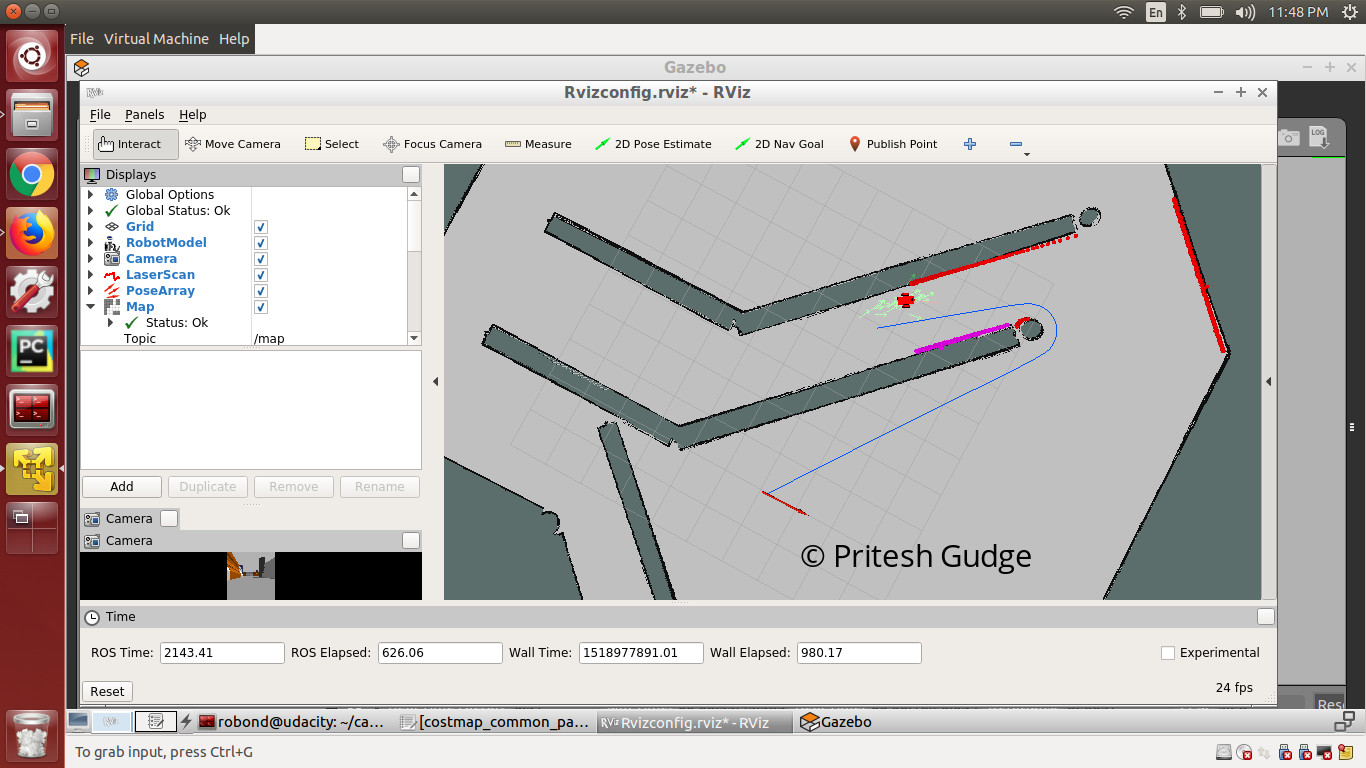
\includegraphics[width=\linewidth]{images/28_attempt2goal_mid1_bm}
      \caption{Benchmark model Intermediate Position 1}
      \label{fig:benchresult3}
\end{figure}


\begin{figure}[thpb]
      \centering
      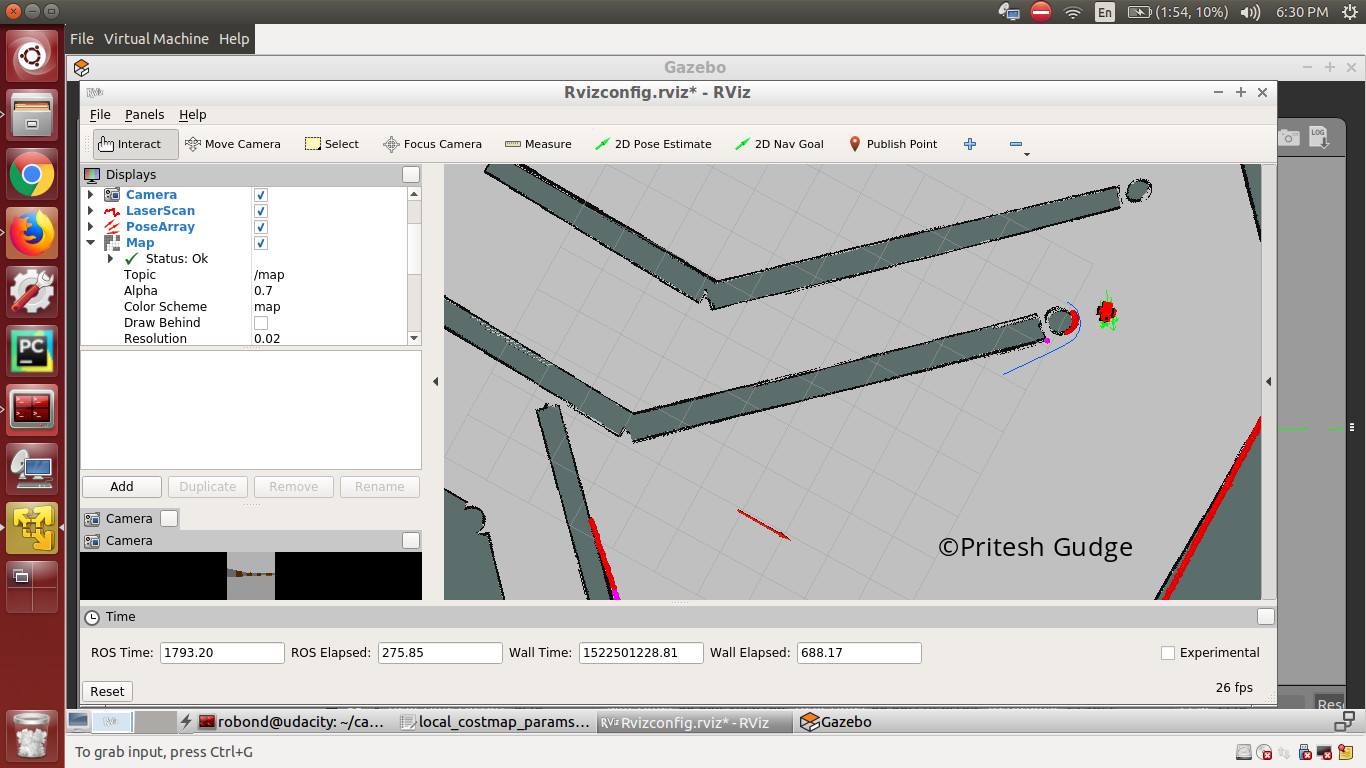
\includegraphics[width=\linewidth]{images/img3_bm}
      \caption{Benchmark model Intermediate Position 2}
      \label{fig:benchresult4}
\end{figure}

\begin{figure}[thpb]
      \centering
      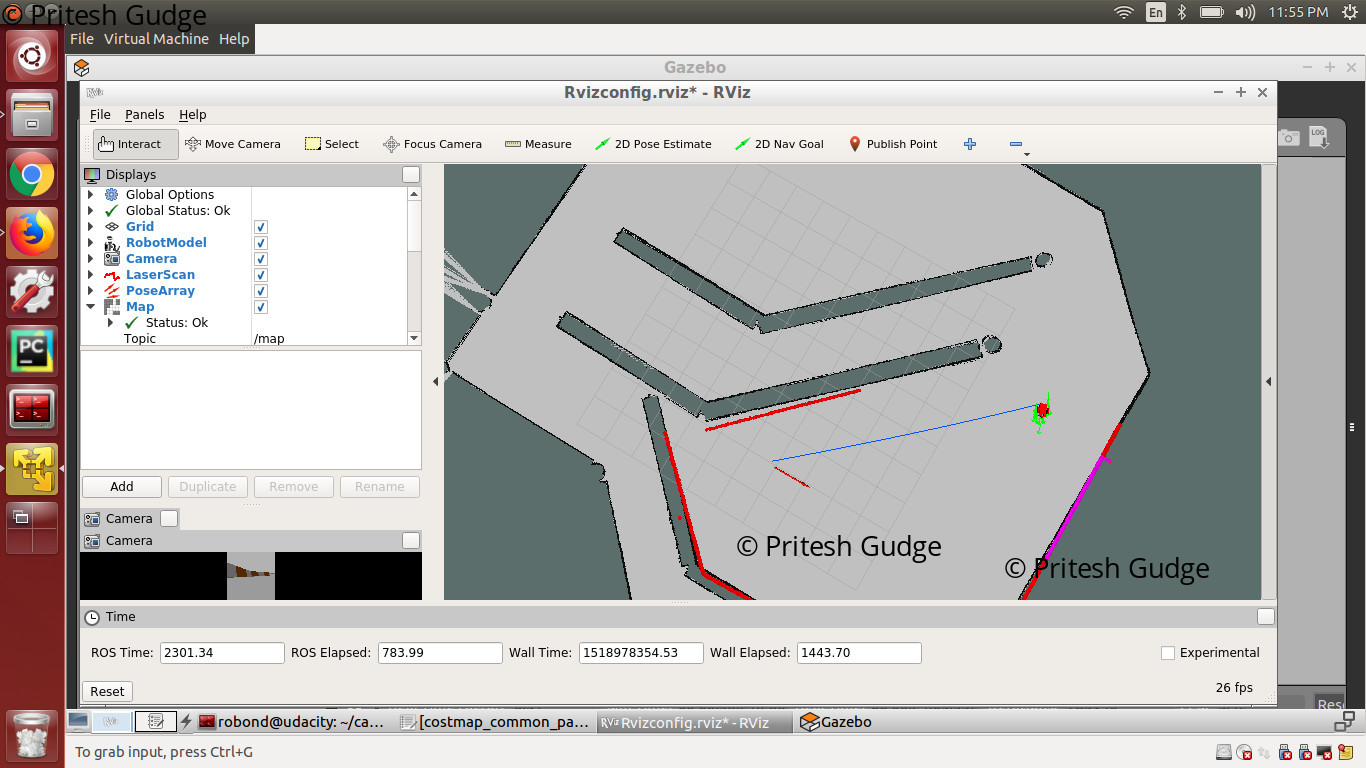
\includegraphics[width=\linewidth]{images/29_goal_attempt_mid3_bm}
      \caption{Benchmark model Position Intermediate Position 3}
      \label{fig:benchresult5}
\end{figure}


\begin{figure}[thpb]
      \centering
      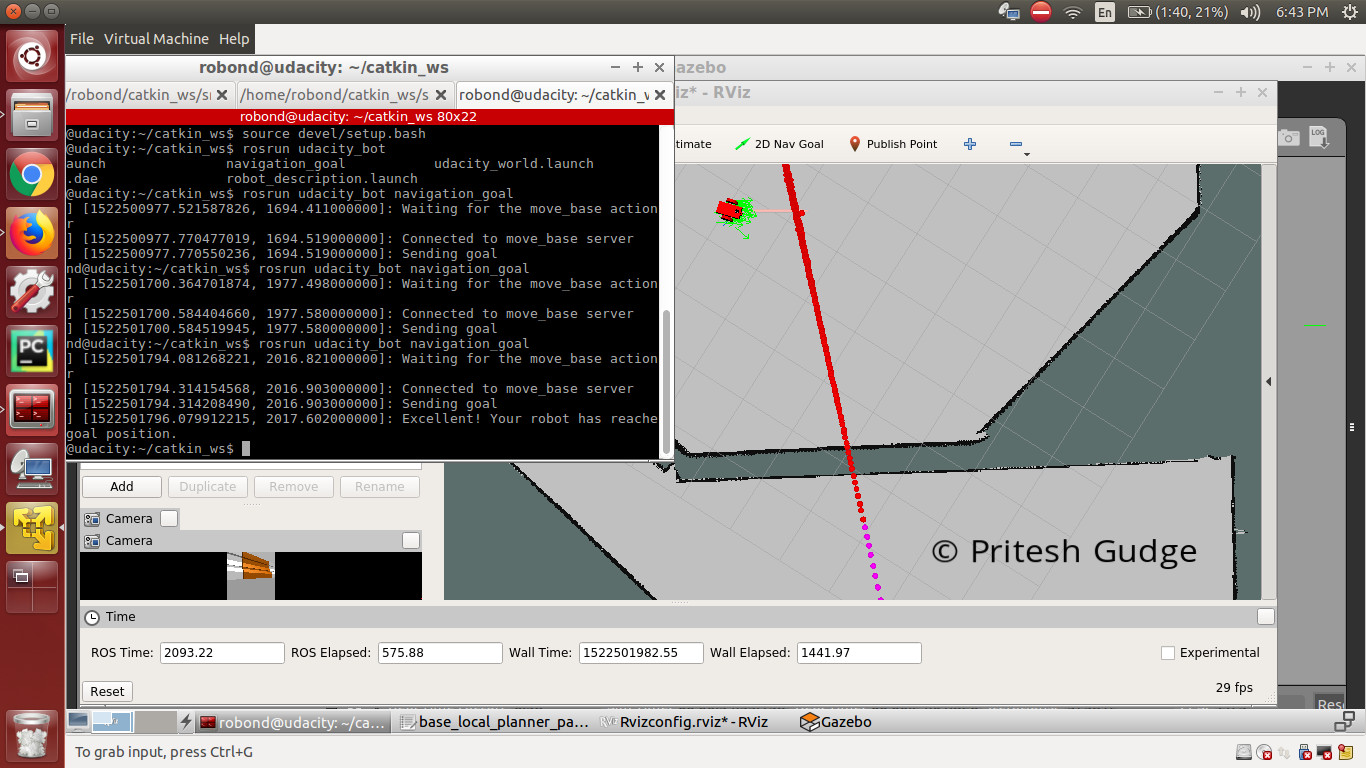
\includegraphics[width=\linewidth]{images/goal}
      \caption{Benchmark model Final Position}
      \label{fig:benchresult1}
\end{figure}

%example for inserting image
\begin{figure}[thpb]
      \centering
      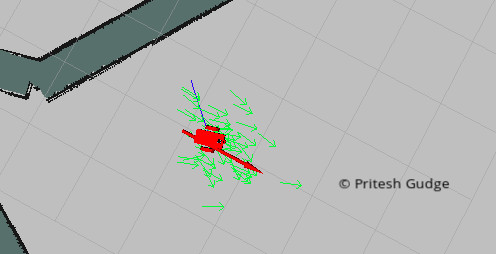
\includegraphics[width=\linewidth]{images/goal_cropped_bm}
      \caption{Benchmark model Final Position}
      \label{fig:benchresult2}
\end{figure}


\subsubsection{Custom}
The custom robot takes the path as shown in figure \ref{fig:customresult1},\ref{fig:customresult2} and figure \ref{fig:customresult3}.
The custom robot reaches near the location as shown in figure \ref{fig:customresult}

\begin{figure}[thpb]
      \centering
      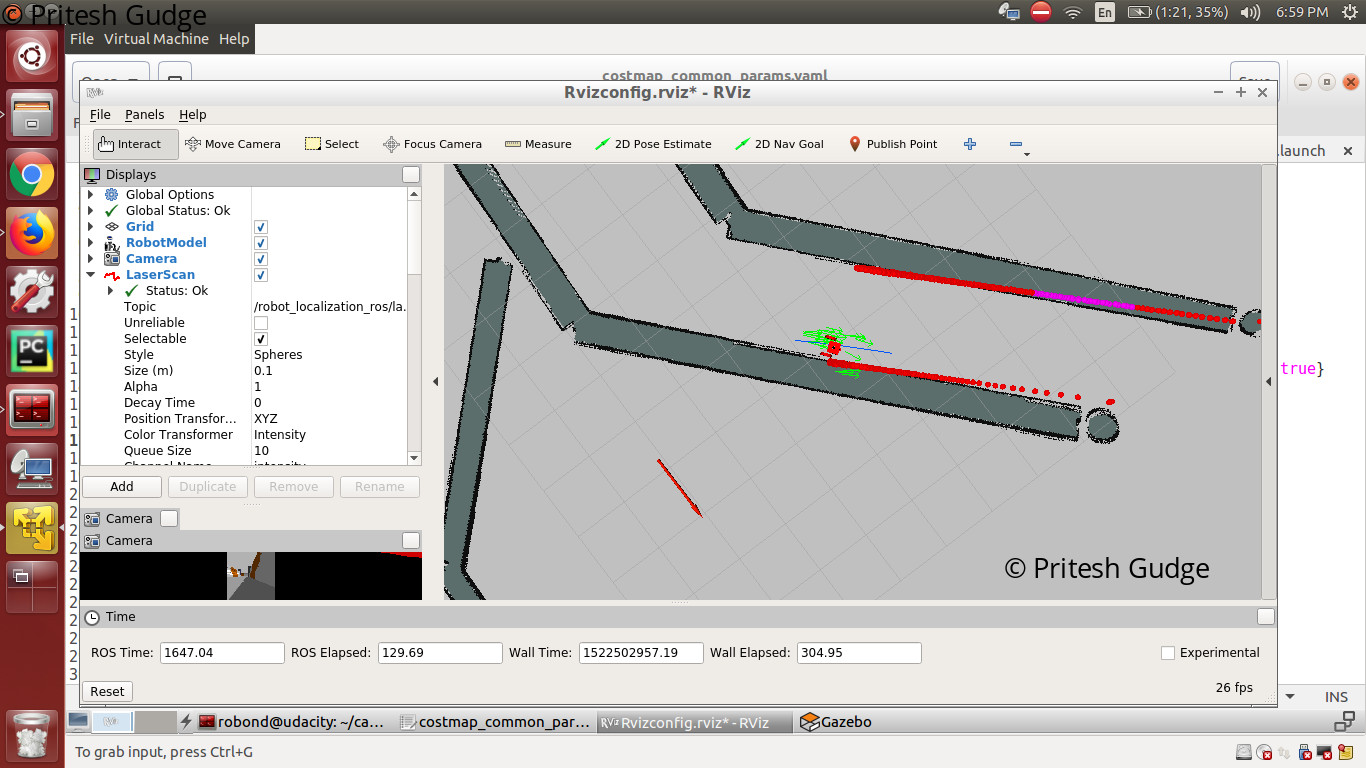
\includegraphics[width=\linewidth]{images/custom1}
      \caption{Custom model Intermediate Position 1}
      \label{fig:customresult1}
\end{figure}


\begin{figure}[thpb]
      \centering
      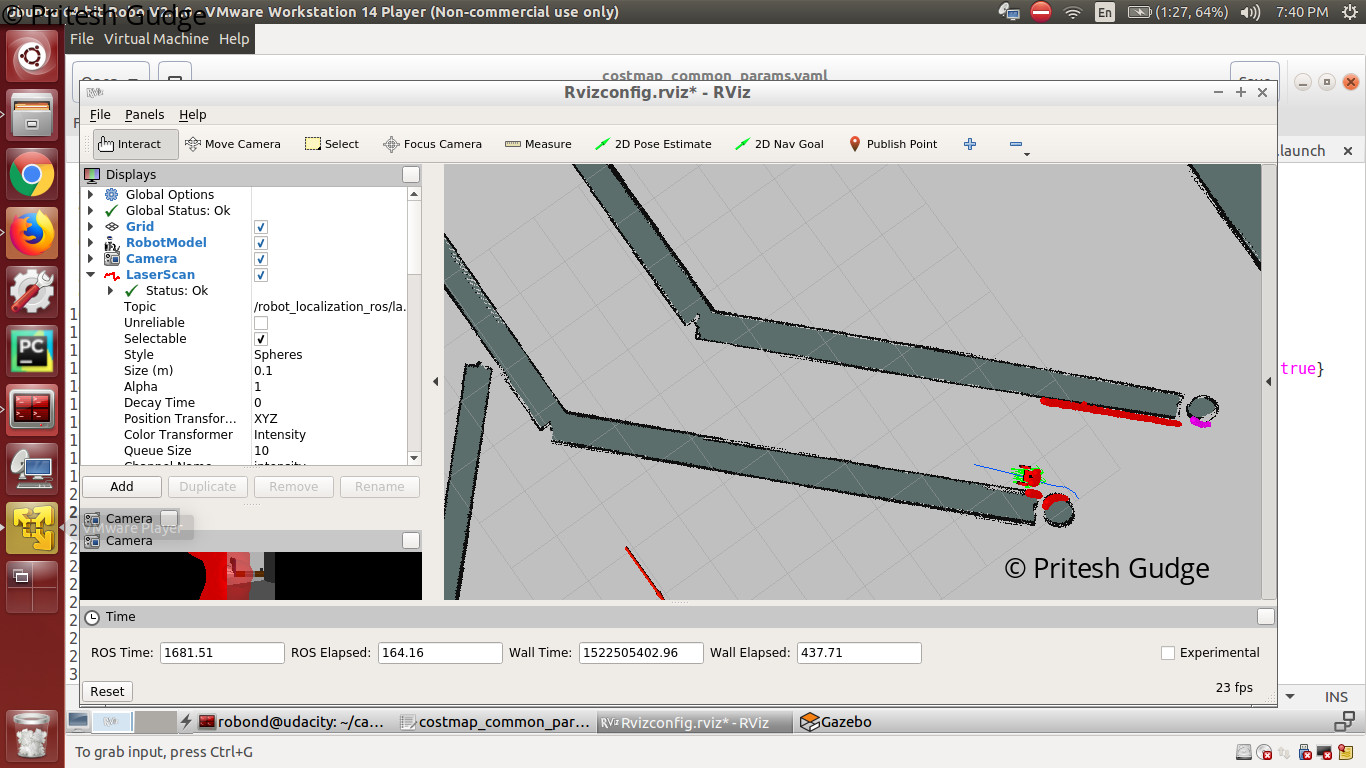
\includegraphics[width=\linewidth]{images/custom3}
      \caption{Custom model Intermediate Position 2}
      \label{fig:customresult2}
\end{figure}


\begin{figure}[thpb]
      \centering
      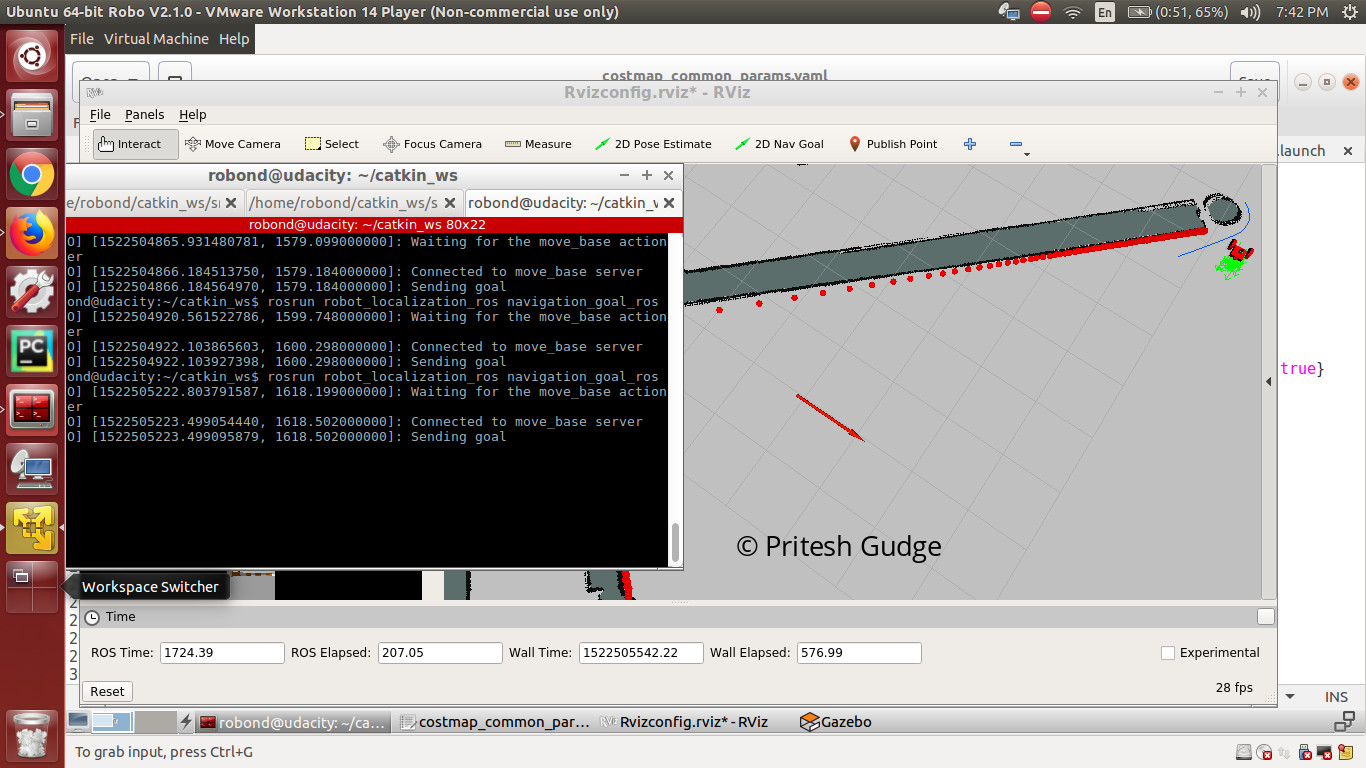
\includegraphics[width=\linewidth]{images/custom4}
      \caption{Custom model Intermediate Position 3}
      \label{fig:customresult3}
\end{figure}
\begin{figure}[thpb]
      \centering
      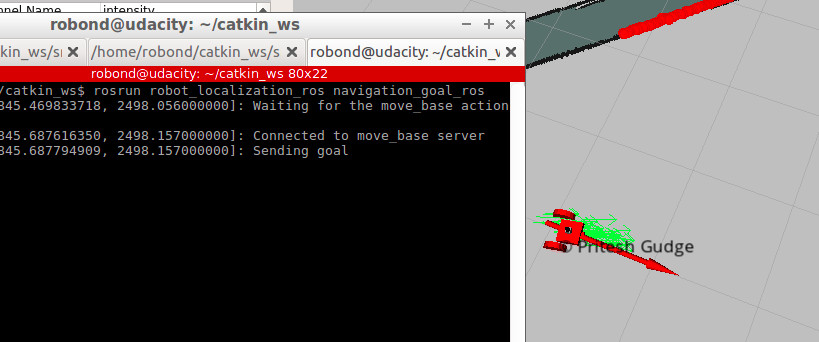
\includegraphics[width=\linewidth]{images/cropped_custom_goal}
      \caption{Custom model Final Position}
      \label{fig:customresult}
\end{figure}


\subsection{Technical Comparison} % only facts
\subsubsection{Layout}
The layout of the robot models are compared in the table \ref{layoutcomparetable}
%example for building table
\begin{table}[h]
\caption{Layout Comparison}
\label{layoutcomparetable}
\begin{center}
\begin{tabular}{|c|c|}
\hline
Benchmark & Custom \\
\hline
2 wheels lateral,2 casters longitudinal & 2 wheels rear,1 caster front \\
\hline
Camera in front & Camera in Front \\
\hline
Laser Range Finder on Top Front & Laser Range Finder on Top Middle \\
\hline
Torque 20 & Torque 20 \\ 
\hline
\end{tabular}
\end{center}
\end{table}

\subsubsection{Parameters}
The main parameters of the models are compared in the table \ref{parametercomparetable}
%example for building table
\begin{table}[h]
\caption{Parameters Comparison}
\label{parametercomparetable}
\begin{center}
\begin{tabular}{|c||c|c|}
\hline
Parameter & Benchmark & Custom \\
\hline
 sim\_time & 2.0 & 1.5 \\
\hline
p\_dist & 2.0 & 2.5 \\
\hline
g\_dist & 3.3 &  1.5\\
\hline
occ\_dist & 1.5 & 1.6\\
\hline
\hline
\end{tabular}
\end{center}
\end{table}

\subsubsection{Performance}
%example for building table
The performances of the models are compared in the table \ref{performancecomparetable}
\begin{table}[h]
\caption{Performance Comparison}
\label{performancecomparetable}
\begin{center}
\begin{tabular}{|c||c|c|}
\hline
Parameter & Benchmark & Custom \\
\hline
Goal Position Time & 12 min & 26 min \\
\hline
Goal Path & Smooth & Oscillating \\
\hline
\end{tabular}
\end{center}
\end{table}

\section{Discussion}

\begin{itemize}
\item \textbf{Performance:} The custom robot performance is poor compared to the bench mark robot.
\item \textbf{Performance Reason:} The design of the custom robot with two wheels in the rear and one caster in the front makes it harder for the custom robot to rotate in position. The center of the custom robot has to go around in a circle for it to be able to change its direction by 180 degrees. There are many reasons for this.  This reduced flexibility especially around bends and in positions where the robot gets stuck causes problems as the localization algorithm does not consider the layout of the robot while estimating the measurements and pose.  

\item \textbf{Kidnapped Robot Situation}: The detection of kidnapped robot is
one of the most difficult problems in Monte Carlo localiza-
tion (MCL).This is due to the nature of particle filter used in MCL itself, where the convergence  process of hypotheses (called particles) causes the absence of particles in some areas, leading to a localization failure if the robot is kidnapped to that area\cite{kidnap}.
In augmented MCL(AMCL)\cite{amclpaper}, random particles are injected in
each iteration so that the possibility of particles’ absence in kidnapping destination area is reduced. 
AMCL does not clearly draw a line between detection and recovery of kidnapping. This creates a problem when the concern is not only in the re-localization but also the needs to know when the kidnapping really happens, such as in fault detection. This is where AMCL fails\cite{kidnap}.

\item \textbf{Kidnapped Robot Situation Alternate Solution:} The 'Kidnapped Robot' problem could attempted to be solved by storing images, distances and locations of the landmarks eg. Corners, bends, poles and the pose of the robot from which the image is captured. A neural network can be trained on this and the trained model can be used to predict the location of the robot based on the image captured by the camera.
\item \textbf{ Industry Use:} MCL and AMCL could be used in robots which performing picking and putaway operations in a warehouse as in a typical warehouse the layout is known precisely and does not change frequently.

\end {itemize}

\section{Conclusion / Future work}

\subsection{Modifications for Improvement}
The following modifications can be attempted to improve the performance of the custom robot. 
\begin{itemize}
\item \textbf{Base Dimension:} The base dimension can be decreased to allow longer radius of turn and preventing the differential from locking.
\item \textbf{Sensor Location:}The Laser range finder can be placed in the front of the chassis for better measurement precision without the chassis blocking part of the surrounding.
\item \textbf{Additional Sensors:} Additional range finders and cameras can be added to the rear and the sides of the chassis to provide for better estimation in location. 
\end{itemize}

\subsection{Hardware Deployment}
\begin{enumerate}
\item The custom chassis can be built by using a block of wood and the range finder and RGB camera can be bought off the shelf. An off the shelf microcontroller can be bought and used to run the localization on board the robot. Standard Wheels and Differential drive controller can be bought off the shelf. The robot can be assembled using the above components.
\item The sim\_time parameter and the resolution parameters for the local and global costmaps can be controlled based on the precision of the final pose of the robot. For the robot to have precise final pose, it is necessary to deploy a computer with higher configuration of CPU and RAM. 
\end{enumerate}



\bibliography{bib}
\bibliographystyle{ieeetr}

\end{document}